\documentclass[10pt]{article}
\usepackage[usenames]{color} %used for font color
\usepackage{amssymb} %maths
\usepackage{amsmath} %maths
\usepackage[utf8]{inputenc} %useful to type directly diacritic characters
\usepackage{tikz}
\usetikzlibrary{positioning, arrows, calc, backgrounds, fit, decorations.pathmorphing}
\definecolor{grey538}{RGB}{240,240,240}
\usepackage{subcaption}\begin{document}
\begin{align*}\begin{minipage}{.5\textwidth}
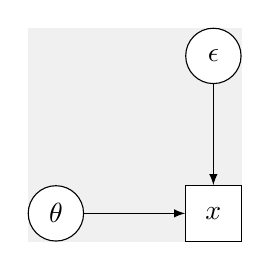
\begin{tikzpicture}[
  grow = right, edge from parent/.style={draw,-latex},
  level distance = 8em, sibling distance = 8em, minimum size = 2em, inner sep = 0,
  scale = 2
]
\tikzstyle {latent} = [draw, shape = circle, fill = white]
\tikzstyle {observed} = [draw, shape = rectangle, fill = white]
% place nodes
\path node (0) [latent] at (0,0) {$\theta$};
\path node (1) [observed] at (1,0) {$x$};
\path node (2) [latent] at (1,1) {$\epsilon$};
% place edges
\foreach \x in {0, 2}
  { \draw [-latex] (\x) -- (1) ; } ;
\begin{scope}[on background layer]
  \node [fill=grey538, fit = (0) (1) (2)] {};
\end{scope}
\end{tikzpicture}
\end{minipage}
\begin{minipage}{.5\textwidth}
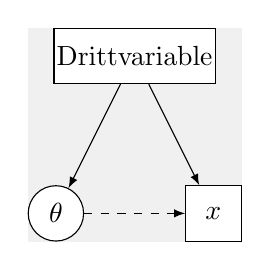
\begin{tikzpicture}[
  grow = right, edge from parent/.style={draw,-latex},
  level distance = 8em, sibling distance = 8em, minimum size = 2em, inner sep = 0,
  scale = 2
]
\tikzstyle {latent} = [draw, shape = circle, fill = white]
\tikzstyle {observed} = [draw, shape = rectangle, fill = white]
% place nodes
\path node (0) [latent] at (0,0) {$\theta$};
\path node (1) [observed] at (1,0) {$x$};
\path node (2) [observed, inner sep = 1] at (.5,1) {Drittvariable};
% place edges
\foreach \x in {0, 1}
  { \draw [-latex] (2) -- (\x) ; } ;
\draw [-latex, ] (0) [dashed] to (1) ; 
\begin{scope}[on background layer]
  \node [fill=grey538, fit = (0) (1) (2)] {};
\end{scope}
\end{tikzpicture}
\end{minipage}\end{align*}
\end{document}